\subsection{Elenco dei casi d'uso - Utente: sviluppatore}	

\subsubsection{UC-15 Ricerca dei dati delle annotazioni}
		\begin{itemize}
			\item \textbf{Attori:} Sviluppatore.
			\item \textbf{Precondizione:} Lo sviluppatore si trova nella vista principale dell'applicazione.
			\item \textbf{Postcondizione:} Lo sviluppatore ottiene una lista delle annotazioni correnti delle frasi.
			\item \textbf{Scenario principale:}
				\begin{enumerate}
					\item Lo sviluppatore accede all'area dei dati.
					\item Lo sviluppatore scrive nella barra di ricerca una sottostringa della frase cercata.
					\item lo sviluppatore seleziona i filtri da usare nella ricerca (UC-15.1).
					\item lo sviluppatore conferma la ricerca
				\end{enumerate}
		\end{itemize}
	
	\subsubsection{UC-15.1 Filtraggio dei dati}	
		\begin{itemize}
			\item \textbf{Attori:} Sviluppatore.
			\item \textbf{Precondizione:} Lo sviluppatore si trova nell'area dati e ha scritto nella barra di ricerca una sottostringa della frase cercata.
			\item \textbf{Postcondizione:} Lo sviluppatore ha indicato i filtri da applicare alla ricerca.
			\item \textbf{Scenario principale:}
				\begin{enumerate}
					\item Lo sviluppatore seleziona il filtro su base temporale (UC-15.1.1).
					\item Lo sviluppatore seleziona il filtro in base agli utenti (UC-15.1.2).
				\end{enumerate}
			\end{itemize}
	\begin{figure}[h]
			\centering
			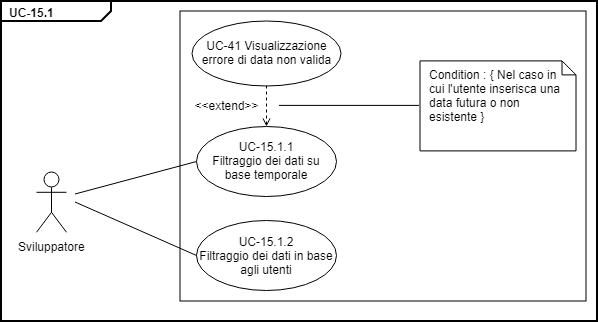
\includegraphics[scale=0.7]{images/UC-15_1.png}
			\caption{UC-15.1 Filtraggio dei dati}
		\end{figure}	
	
	\subsubsection{UC-15.1.1 Filtraggio dei dati su base temporale}	
		\begin{itemize}
			\item \textbf{Attori:} Sviluppatore.
			\item \textbf{Precondizione:} Lo sviluppatore si trova nell'area dati e ha scritto nella barra di ricerca una sottostringa della frase cercata.
			\item \textbf{Postcondizione:} Lo sviluppatore ha indicato il filtro su base temporale della ricerca.
			\item \textbf{Scenario principale:}
				\begin{enumerate}
					\item Lo sviluppatore indica due date che definiscono un intervallo di tempo per restringere la ricerca.
				\end{enumerate}
			\item \textbf{Estensioni:}
				\begin{itemize}
					\item 4.a Se i parametri inseriti dall'utente non sono coerenti viene mostrato un messaggio di errore (UC-41).
				\end{itemize}		
		\end{itemize}
			
	\subsubsection{UC-41 Visualizzazione messaggio di errore: data non valida}
		\begin{itemize}					
			\item \textbf{Attori:} Sviluppatore.
			\item \textbf{Precondizione:} Lo sviluppatore ha indicato un intervallo di tempo non valido.
			\item \textbf{Postcondizione:} Lo sviluppatore torna all'area dati.
			\item \textbf{Scenario principale:}
				\begin{enumerate}
					\item Lo sviluppatore visualizza un messaggio di errore "L'intervallo di tempo indicato non è valido".
				\end{enumerate}	
		\end{itemize}					
	
		\begin{figure}[h]
			\centering
			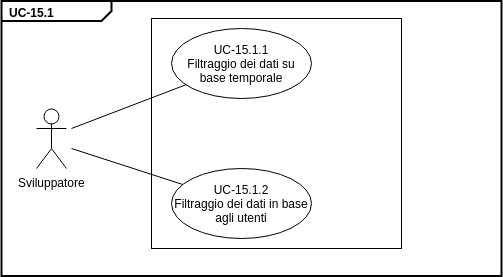
\includegraphics[scale=0.7]{images/UC-15_1_1.png}
			\caption{UC-15.1.1 Filtraggio dei dati su base temporale e UC-15.1.2 Filtraggio dei dati in base agli utenti}
		\end{figure}	
				
	\subsubsection{UC-15.1.2 Filtraggio dei dati in base agli utenti}	
		\begin{itemize}
			\item \textbf{Attori:} Sviluppatore.
			\item \textbf{Precondizione:} Lo sviluppatore si trova nell'area dati e ha scritto nella barra di ricerca una sottostringa della frase cercata.
			\item \textbf{Postcondizione:} Lo sviluppatore ha indicato il filtro in base agli utenti.
			\item \textbf{Scenario principale:}
				\begin{enumerate}
					\item Lo sviluppatore indica l'inclusione o l'esclusione di un utente.
					\item Lo sviluppatore indica gli utenti da includere o escludere.
				\end{enumerate}
		\end{itemize}
		
	\subsubsection{UC-16 Visualizzazione dei dati di una annotazione di una frase}
		\begin{itemize}
			\item \textbf{Attori:} Sviluppatore.
			\item \textbf{Precondizione:} Lo sviluppatore si trova nell'area dati e ha a disposizione i risultati della ricerca delle annotazioni.
			\item \textbf{Postcondizione:} Lo sviluppatore legge i dati di una annotazione di una frase.
			\item \textbf{Scenario principale:}
				\begin{enumerate}
					\item Lo sviluppatore seleziona una annotazione.
					\item Lo sviluppatore visualizza data, utente e soluzione proposta
				\end{enumerate}
		\end{itemize}
	
	\subsubsection{UC-17 Visualizzazione storico}		
		\begin{itemize}
			\item \textbf{Attori:} Sviluppatore.
			\item \textbf{Precondizione:} Lo sviluppatore si trova nell'area dati e ha a disposizione i risultati della ricerca delle annotazioni.
			\item \textbf{Postcondizione:} Lo sviluppatore visualizza lo storico delle annotazioni ottenute dalla ricerca precedente.
			\item \textbf{Scenario principale:}
			\begin{enumerate}
				\item Lo sviluppatore seleziona l'opzione "vedi storico".
			\end{enumerate}
		\end{itemize}	
		
	\subsubsection{UC-18 Ordinamento dei risultati}
		\begin{itemize}
			\item \textbf{Attori:} Sviluppatore.
			\item \textbf{Precondizione:} Lo sviluppatore si trova nell'area dati con i risultati della ricerca effettuata.
			\item \textbf{Postcondizione:} Lo sviluppatore ottiene la lista precedente ordinata in base alle scelte effettuate.
			\item \textbf{Scenario principale:}
				\begin{enumerate}
					\item Lo sviluppatore sceglie il parametro secondo il quale ordinare i risultati (alfabetico, frequenza, ultima correzione, utente).
					\item Lo sviluppatore conferma l'ordinamento scelto.
				\end{enumerate}
		\end{itemize} 
	
	\subsubsection{UC-19 Download dei dati raccolti}
		\begin{itemize}
			\item \textbf{Attori:} Sviluppatore.
			\item \textbf{Precondizione:} Lo sviluppatore si trova nell'area dati con i risultati della ricerca effettuata.
			\item \textbf{Postcondizione:} Lo sviluppatore ottiene un file \texttt{.txt} con i dati dei risultati precedentemente trovati.
			\item \textbf{Scenario principale:}
				\begin{enumerate}
					\item Lo sviluppatore richiede il download dei dati.
					\item Lo sviluppatore decide il path in cui il file viene salvato.
					\item Lo sviluppatore esegue il salvataggio.
				\end{enumerate}
			\item \textbf{Estensioni:}
				\begin{itemize}
					\item 2.a Se il path indicato è inesistente, viene visualizzato un messaggio di errore (UC-42).
				\end{itemize}
		\end{itemize}

	\subsubsection{UC-42 Visualizzazione messaggio di errore: path inesistente}
		\begin{itemize}					
			\item \textbf{Attori:} Sviluppatore.
			\item \textbf{Precondizione:} Lo sviluppatore ha indicato un path non esistente.
			\item \textbf{Postcondizione:} Lo sviluppatore torna all'area dati.
			\item \textbf{Scenario principale:}
				\begin{enumerate}
					\item Lo sviluppatore visualizza un messaggio di errore "Path inesistente".
				\end{enumerate}	
		\end{itemize}					

		\begin{figure}[h]
			\centering
			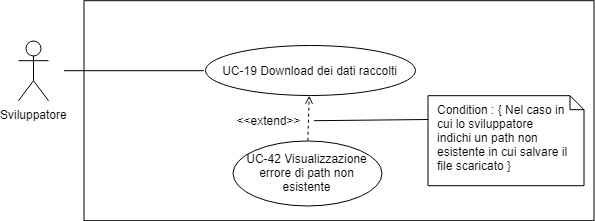
\includegraphics[scale=0.7]{images/UC-19.png}
			\caption{UC-19 Download dei dati raccolti}
		\end{figure}	
		
	\subsubsection{UC-20 Download di un dataset}
		\begin{itemize}
			\item \textbf{Attori:} Sviluppatore.
			\item \textbf{Precondizione:} Lo sviluppatore si trova nell'area dati con i risultati della ricerca effettuata.
			\item \textbf{Postcondizione:} Lo sviluppatore ottiene il dataset in un file \texttt{.txt}.
			\item \textbf{Scenario principale:}
			\begin{enumerate}
				\item Lo sviluppatore richiede il download del dataset, contenente l'input della fase di train del software di apprendimento automatico.
				\item Lo sviluppatore decide il path in cui il file viene salvato.
				\item Lo sviluppatore esegue il salvataggio.
			\end{enumerate}
			\item \textbf{Estensioni:}
				\begin{itemize}
					\item 2.a Se il path indicato è inesistente, viene visualizzato un messaggio di errore (UC-42).
				\end{itemize}
		\end{itemize}
	
	\subsubsection{UC-21 Download di un modello}
		\begin{itemize}
			\item \textbf{Attori:} Sviluppatore.
			\item \textbf{Precondizione:} Lo sviluppatore si trova nella vista con le informazioni del modello selezionato.
			\item \textbf{Postcondizione:} Lo sviluppatore ottiene un file binario con il modello.
			\item \textbf{Scenario principale:}
			\begin{enumerate}
					\item Lo sviluppatore richiede il download del modello.
					\item Lo sviluppatore decide il path in cui il file viene salvato.
					\item Lo sviluppatore esegue il salvataggio.
				\end{enumerate}
			\item \textbf{Estensioni:}
				\begin{itemize}
					\item 2.a Se il path indicato è inesistente, viene visualizzato un messaggio di errore (UC-42).
				\end{itemize}
		\end{itemize}
		
		\begin{figure}[h]
			\centering
			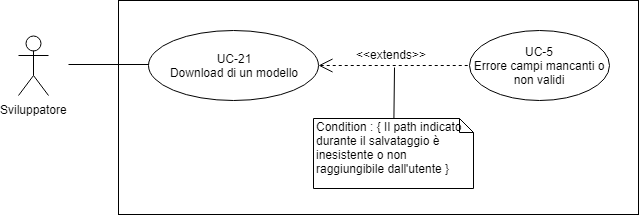
\includegraphics[scale=0.7]{images/UC-21.png}
			\caption{UC-21 Download di un modello}
		\end{figure}		
		
	\subsubsection{UC-22 Creazione di un modello}		
		\begin{itemize}
			\item \textbf{Attori:} Sviluppatore.
			\item \textbf{Precondizione:} Lo sviluppatore si trova nell'area dati.
			\item \textbf{Postcondizione:} Lo sviluppatore aggiunge un modello alla piattaforma.
			\item \textbf{Scenario principale:}
			\begin{enumerate}
				\item Lo sviluppatore seleziona la funzione di aggiunta di un modello.
				\item Lo sviluppatore inserisce il file che contiene un dataset.
				\item Lo sviluppatore conferma la creazione.
			\end{enumerate}
			\item \textbf{Estensioni:}
				\begin{itemize}
					\item 4.a Se il dataset fornito ha un formato errato, viene visualizzato un messaggio di errore (UC-43).
				\end{itemize}
		\end{itemize}
		
		\begin{figure}[h]
			\centering
			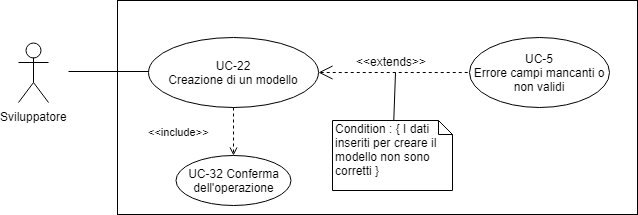
\includegraphics[scale=0.7]{images/UC-22.png}
				\caption{UC-22 Creazione di un modello}
		\end{figure}	
	
	\subsubsection{UC-43 Visualizzazione errore: formato del dataset errato}	
	
	\subsubsection{UC-44 Cambio modello}
	
	